\chapter{Interferometric stabilisation of reservoir cavity}

\label{ch-stabilisation}

%%%%%%%%%% INTRODUCTION %%%%%%%%%%

\section{Introduction}

In this introductory section, the concept of interferometry is presented. As the name of the chapter suggests, this technique is used to stabilise the reservoir cavity. The reason why an optical cavity needs stabilisation will appear clearer later, but basically, this is due to the fact that light is a wave and that it can interfere with itself inside the cavity. The interferences can be constructive, destructive, or can behave in any intermediate way. Moreover, it will be shown that the interferometric properties are wavelength dependent. Since several wavelengths coexist inside the reservoir, this gives a first glimpse on the complexity entailing its stabilisation. To gain some insight on interferometry, and before moving on to the study of an actual ring cavity, the features of the well known \gls{fp} interferometer are recalled. After that, it is shown that the properties studied for the \gls{fp} can be translated to ring cavities with close to no modification. Finally, under the light of the basic notions of interferometry developed, the difficulties linked to the stabilisation of the reservoir cavity, which is at the heart of the scheme introduced in this thesis, are presented.

%%% FABRY-PEROT INTERFEROMETER %%%

\subsection{Fabry-Perot interferometer}

The \gls{fp} plays an important role in modern optics as it is really ubiquitous. This can be explained by the fact that, despite its great simplicity, it can reach good performance using high reflectivity mirrors, which can be produced using nowadays technologies. In practice, a \gls{fp} cavity is simply made of two facing mirrors as can be viewed on figure \ref{fp}. On this figure, one can see the two mirrors, represented by the vertical black lines, and the different electric fields. The resonance condition, namely the regime where the transmitted electric field $E_{\text{t}}$ is maximum, can be seen intuitively as a situation where the intra-cavity field $E_1$ is in phase with the incident field $E_{\text{in}}$, which leads to the build up of a very intense intra-cavity electric field. On the other hand, the anti-resonance condition is met when $E_{\text{in}}$ and $E_1$ are out of phase. The transmissivity of the \gls{fp} interferometer, which is defined as the ratio $|E_{\text{t}}|^2/|E_{\text{in}}|^2$, is given by \cite{Perot1899}:

\begin{equation}
	\mathcal{T}(\omega) = \frac{1}{1+\mathcal{F}\sin^2{\left(\frac{\omega}{\text{FSR}}\right)}}
	\label{transmissivity}
\end{equation}

In this expression, $\mathcal{F}$ is the finesse of the cavity, $\omega$ is the angular frequency of the incident electric field, and FSR is the \acrlong{fsr} of the cavity. In a stationary regime, the energy inside the cavity does not evolve, therefore the energy carried by the incident electric field $E_{\text{in}}$ can either be transmitted or reflected, which implies that the reflectivity of the cavity which is defined as the ratio $|E_{\text{ref}}|^2/|E_{\text{in}}|^2$ is simply given by:

\begin{equation}
	\mathcal{R}(\omega) = 1 - \mathcal{T}(\omega)
	\label{reflectivity}
\end{equation}

\begin{figure}[h]
	\centering
	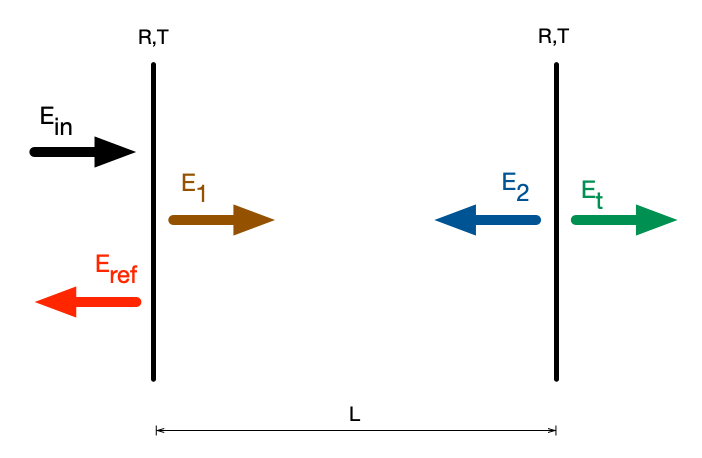
\includegraphics[width=.65\textwidth]{fp}
	\caption{Schematic representation of a \acrlong{fp} interferometer. $E_{\text{in}}$ is the incident electric field, $E_{\text{ref}}$ is the reflected electric field, $E_{\text{t}}$ is the transmitted electric field, $E_{1}$ is the intra-cavity electric field propagating from left to right, $E_{2}$ is the intra-cavity electric field propagating from right to left, $R$ and $T$ are the reflectivity and transmissivity of the mirrors and $L$ is the distance between them.}
	\label{fp}
\end{figure}

On figure \ref{fp-tf}, the transmissivity (right) and reflectivity (left) can be viewed. These graphs are made of peaks which are distant of the \gls{fsr} in the spectral domain. Recalling that $\text{FSR} = c/2nL$, one can see that the \gls{fsr} is linked to the length of the cavity, with $c$ the speed of light and $n$ the refractive index of the medium that could be present between the two mirrors ($nL$ is the optical path). The finesse $\mathcal{F}$ is related to the width of the peaks and depends on the reflectivity of the mirrors as $\mathcal{F} = 4R/(1-R)^2$. As the reflectivity of the mirrors tends to 1, the finesse tends to infinity, and the peaks get infinitely narrow. On the other hand, with a lower reflectivity, more energy can leak out of the cavity even outside the resonance condition. Seeing the broadening of the peaks as energy leakage will be useful when drawing a parallel between \gls{fp} and ring cavity interferometers.

\begin{figure}[h]
	\centering
	\begin{subfigure}{.5\textwidth}
		\centering
		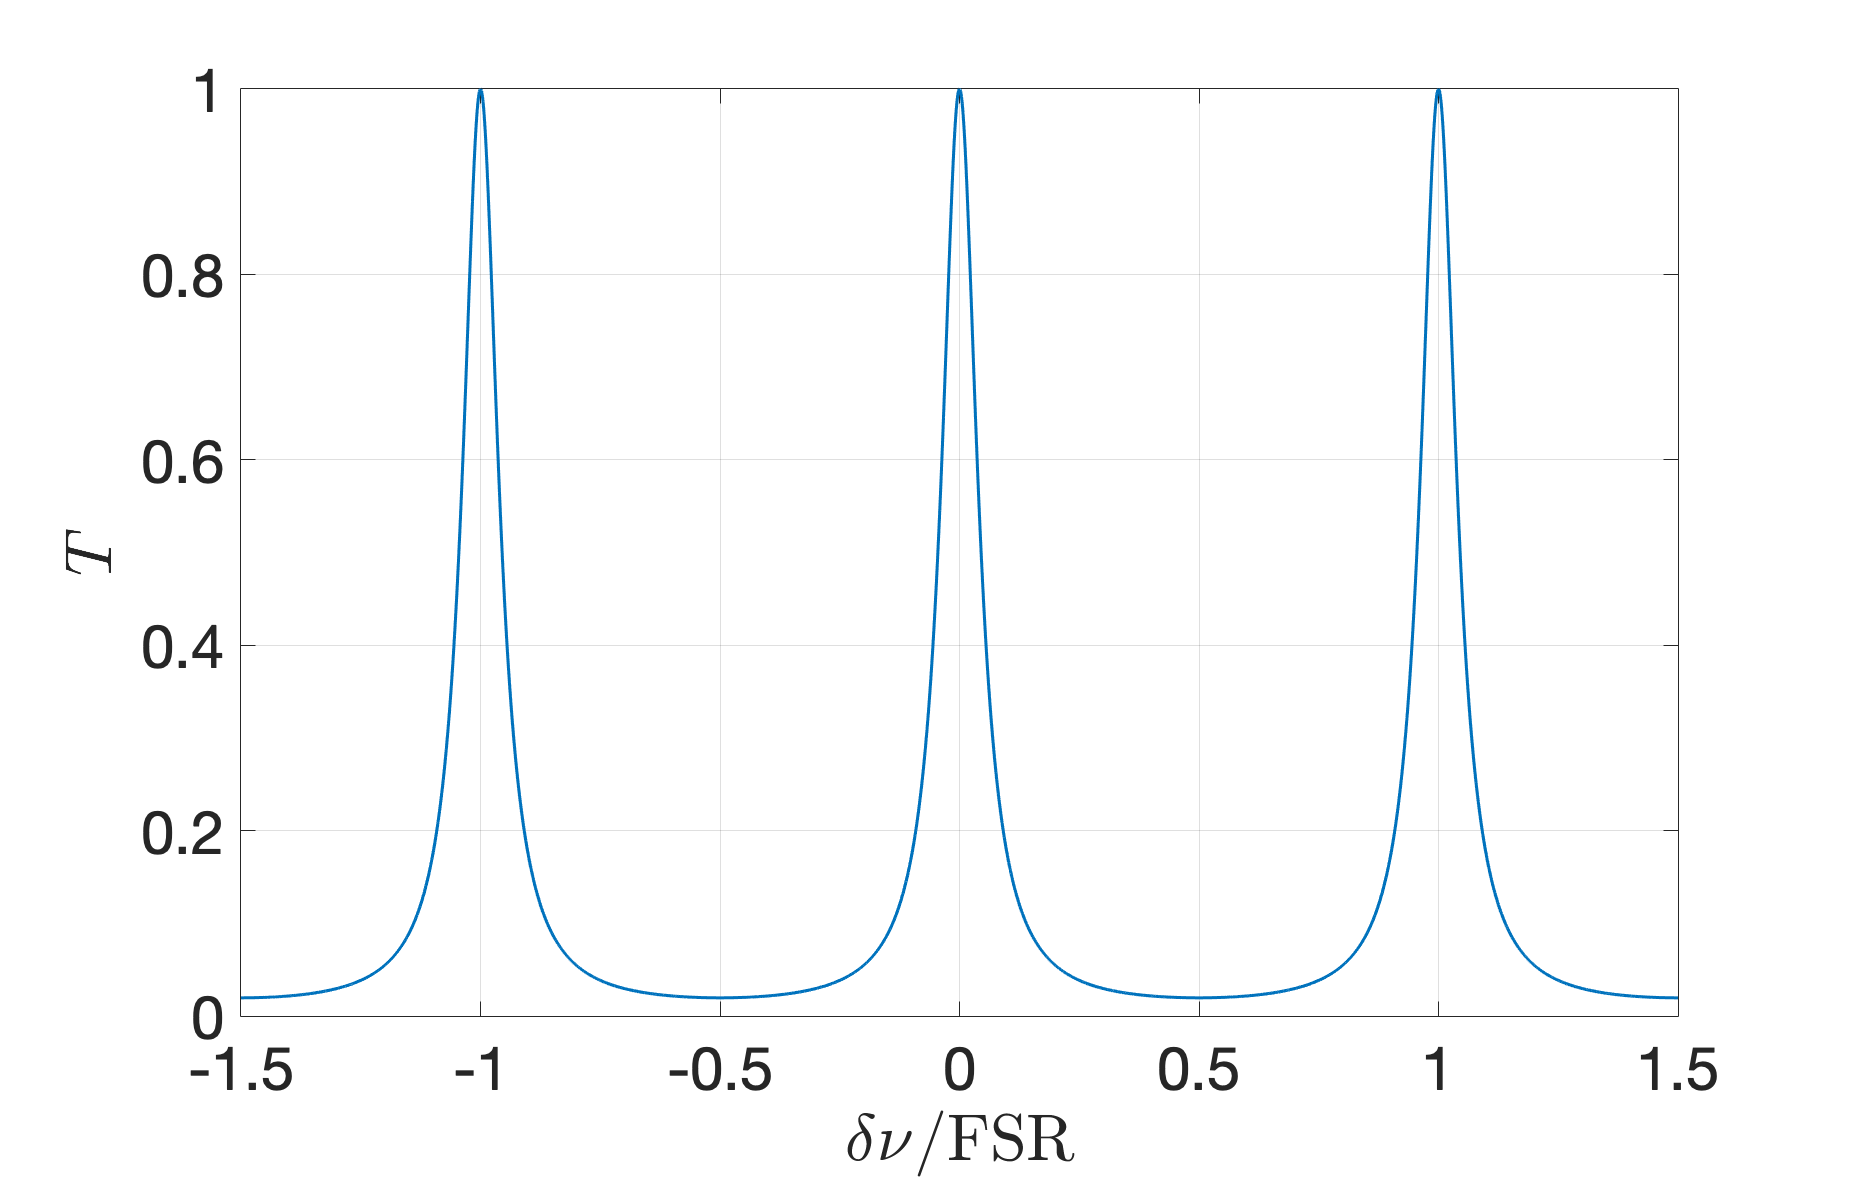
\includegraphics[width=\textwidth]{fp-trans-tf}
	\end{subfigure}%
	\begin{subfigure}{.5\textwidth}
		\centering
		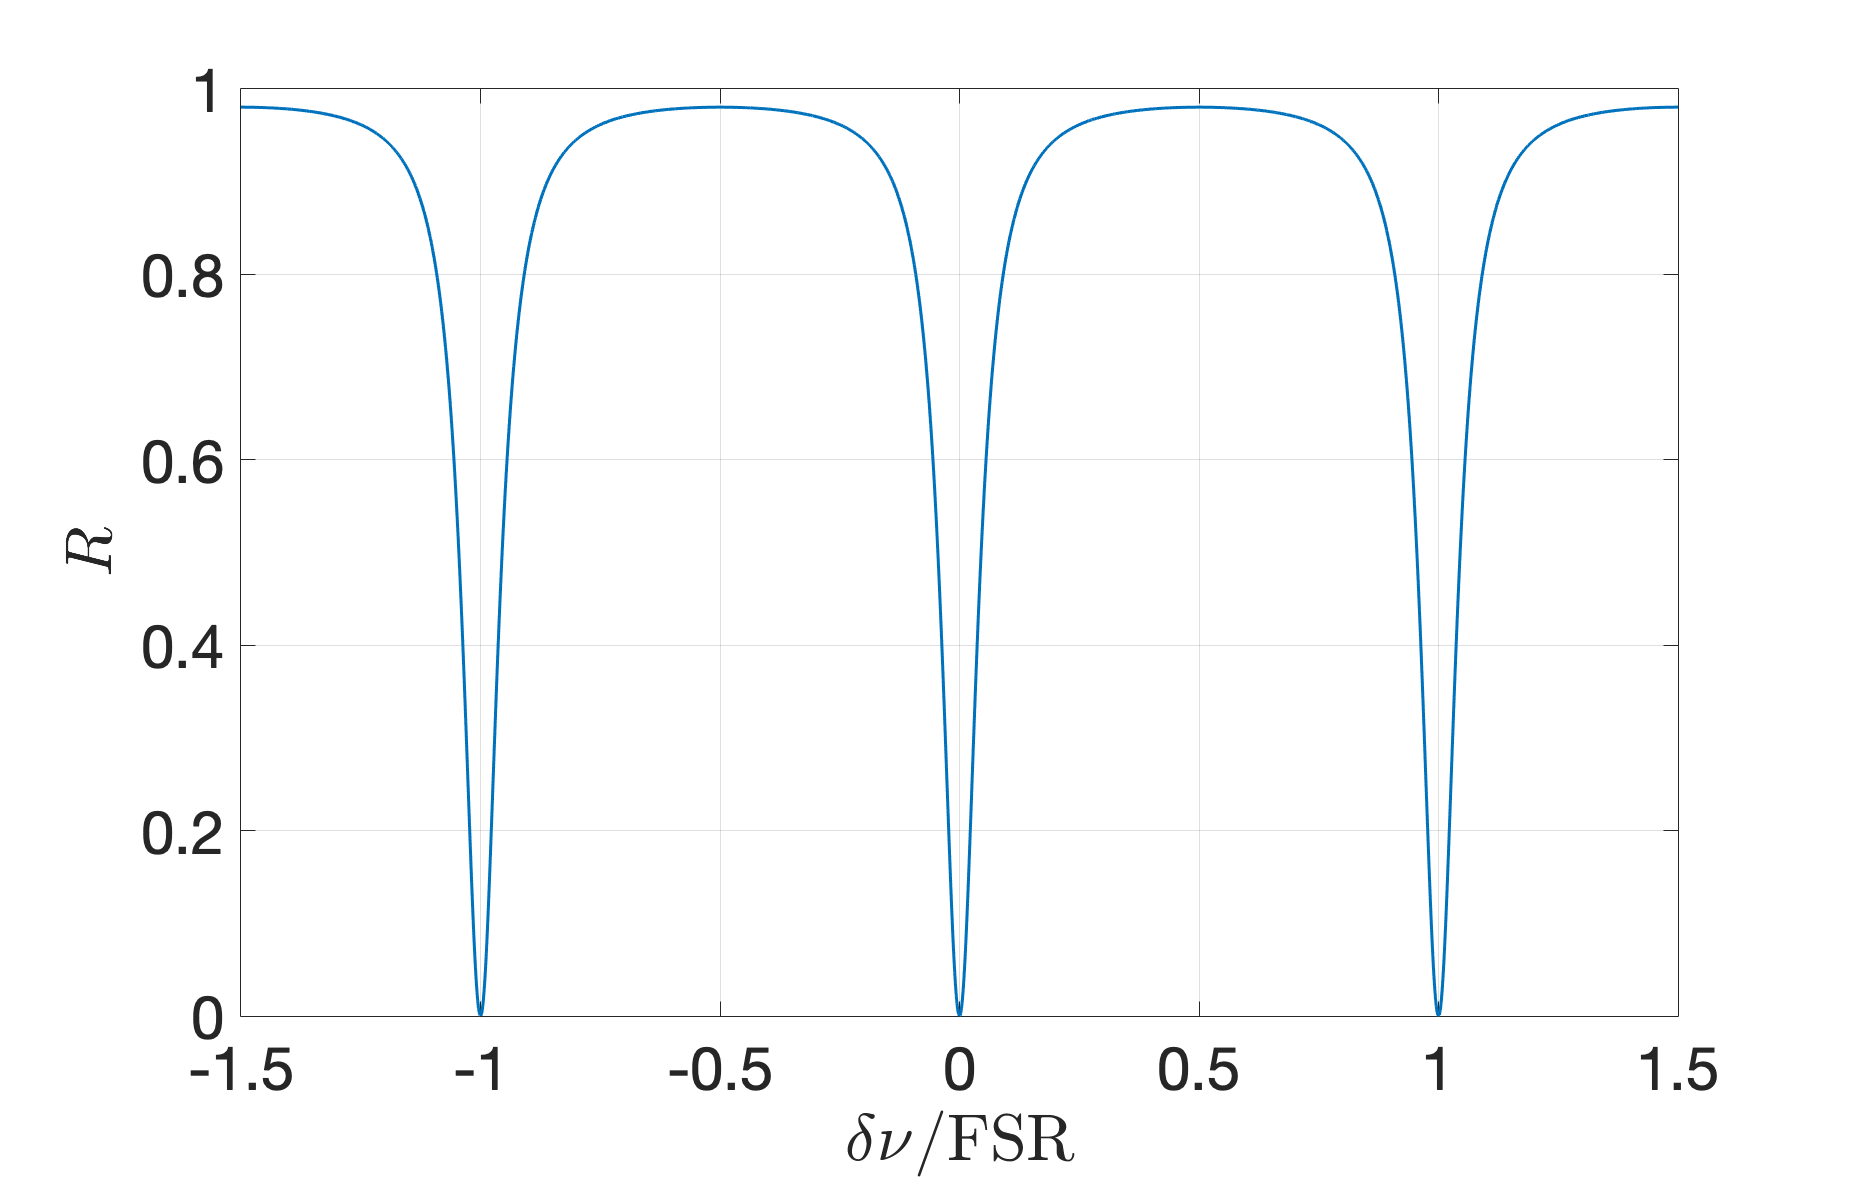
\includegraphics[width=\textwidth]{fp-ref-tf}
	\end{subfigure}
	\caption{Transmissivity $\mathcal{T}$ (left) and reflectivity $\mathcal{R}$ (right) of the cavity. Finesse $\mathcal{F}=50$. $\delta \nu$ denotes the deviation from a resonant frequency.}
	\label{fp-tf}
\end{figure}

Equation \eqref{transmissivity} and \eqref{reflectivity} indicate that $\mathcal{T}$ and $\mathcal{R}$ depend on $\omega/\text{FSR}$. This value can be rearranged as:

\begin{equation}
	\frac{\omega}{\text{FSR}} = kL = \phi
\end{equation}

Where $k$ is the wave number defined as $n \omega/c$ and $\phi$ is the phase acquired by the electric field when propagating along the cavity. Therefore, by measuring the transmitted or reflected power, one can gain information about the phase (modulo $\pi$, because the periodicity of $\mathcal{T}$ and $\mathcal{R}$ in the phase domain is $\pi$) of the electric field. This is the idea underlying interferometry.

%%% RING CAVITY %%%

\subsection{Ring cavity}

A ring cavity exhibits the same behaviour as a \gls{fp} interferometer. The structure of a ring cavity interferometer is displayed on figure \ref{cavity_vs_fp}. This is a fibre-based setup in which the incident electric field $E_{\text{in}}$ penetrates the cavity from the left through a coupler. $E_{\text{ref}}$ denotes the electric field exiting the cavity and $E_1$ and $E_2$ refer to the fields entering and leaving the fibre loop, respectively. The nomenclature for the fields was chosen in such a way that the analogy with the \gls{fp} cavity can be understood. Indeed, one could see the coupler acting as the leftmost mirror from the figure \ref{fp}, and the fibre loop as the one on the right side because it turns $E_1$ into $E_2$ and dissipates energy through fibre losses, whereas for the mirror it was by leakage out of the cavity.

\begin{figure}[h]
	\centering
	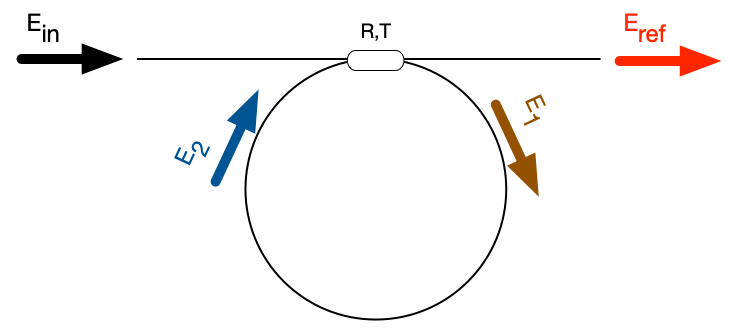
\includegraphics[width=.7\textwidth]{cavity_vs_fp}
	\caption{Schematic view of a ring cavity}
	\label{cavity_vs_fp}
\end{figure}

Because of the similarities between ring cavities and \glspl{fp}, the former show the same transmissivity and reflectivity as the latter. Therefore, by measuring the reflected power, one can determine the phase acquired by the electric field inside the cavity.

%%% Challenge %%%

\subsection{Challenge}

The basic principle of interferometry has been introduced through the presentation of the \gls{fp} interferometer, and in the discussion that followed, it has been shown that a ring cavity, such as the reservoir cavity studied in this thesis, can be used as an interferometer. Moreover, it has also been showed that $\mathcal{R}$ depends on the frequency (or wavelength) and on the length of the cavity and that the phase acquired by the incident electric field after one round trip could be determined by studying the reflected power.\\

In the reservoir cavity, many different wavelengths coexist because they encode the different neurons. Furthermore, after each round trip, the phase acquired by each neuron should be a constant, as shown on equation \eqref{model-reservoir}. Recalling the phase matrix $\mathbf{\Phi}$ defined in equation \eqref{phase-matrix}, the phase factor multiplying the $k^{\text{th}}$ neuron is given by $\Phi_{kk} = \exp{(i\phi_k)}$.	The phase $\phi_k$ is given by:

\begin{equation}
	\phi_k = \beta(\omega+k\Omega) L
\end{equation}

With $\beta$ the fibre wave number, $\omega+k\Omega$ the angular frequency of the $k^{\text{th}}$ neuron and $L$ the length of the fibre loop. Because $k\Omega \ll \omega$, the wave number can be Taylor expanded: 

\begin{equation}
	\beta(\omega+k\Omega) = \beta(\omega) + \left. \frac{\partial\beta}{\partial\omega}\right\rvert_\omega k\Omega + \mathcal{O}\left((k\Omega)^2\right)
\end{equation}

By rewriting $\beta(\omega)$ and $\partial\beta/\partial\omega\rvert_\omega$ as $\beta_0$ and $\beta_1$ as it is often done in the literature, the acquired phase is given by:

\begin{equation}
	\phi_k \approx \beta_0 L + k \beta_1 \Omega L = \phi_0 + k \phi_1
\end{equation}

This means that if $\phi_1$ is an integer multiple of $\pi$, the phase factor multiplying all the neurons will be the same up to a sign:

\begin{equation}
	e^{i(\phi_0+k\phi_1)} = e^{i\phi_0}e^{ikm\pi} =(-1)^{km} e^{i\phi_0}, \quad m \in \mathbb{Z}
\end{equation}

A periodicity of $\pi$ and not $2\pi$ is considered here, because as claimed before, an interferometer can only inform about a phase modulo $\pi$. Looking for an acquired phase equal to $\pi$ is the approximately the same as taking a modulation frequency $\Omega$ for the \gls{pm} which is an integer multiple of the \gls{fsr}. Indeed, by considering $\beta_1 \approx n/c$, one can find:

\begin{equation}
	\beta_1 \Omega L \approx \frac{\Omega n L}{c} = m\pi \longrightarrow \Omega \approx \frac{m\pi c}{n L} = m2\pi ~\text{FSR}
\end{equation}

This is a legitimate assumption given the fact that in the region of interest the curve of $\beta(\omega)$ computed using the Sellmeier relations \cite{Bruckner,malitson1965interspecimen} is very linear.\\

It is not critical to modulate the phase at an angular frequency $\Omega$ which is an integer multiple of the \gls{fsr}, the reservoir can in fact operate in different regimes. Those considerations were presented to better understand the physics underlying the phase management of the reservoir.\\

The main practical challenge regarding the reservoir concerns its stabilisation. The reservoir has to be stabilised because during its operation, external elements disturb it, which deteriorates the performances and even make it unusable in the worst case. The perturbations acting on the reservoir can come from various sources, such as mechanical constraints or temperature changes for example, and can induce a phase fluctuation. This is where interferometric stabilisation comes into play. Indeed, by measuring the power reflected by the reservoir, one can infer the current phase and take the appropriate action to maintain it at a setpoint. This can be achieved using classical regulation strategies, such as a \gls{pid} regulator. Elements of regulation will be presented later. Furthermore, this needs to be performed for all the neurons at the same time. This explains why different elements regarding the relative phases between the different neurons were discussed in the previous paragraph. Finally, the last technological difficulty associated to this scheme is the fact that the electric field used to stabilise the cavity is modulated in amplitude to carry the data to be processed by the reservoir. Indeed, a regulator struggles to differentiate a variation in the reflected power due to a phase fluctuation or to the modulation of the incident field.

%%%%%%%%%% EXPERIMENTAL SETUP %%%%%%%%%%

\section{Experimental setup}

In this section, the experimental setup employed to physically implement the \gls{wdm} \gls{prc} is presented. First, it is detailed based with the help of the schematic representation of figure \ref{exp-setup}. Then, technical data about the devices involved in the experiment are given.

\begin{figure}[h]
	\centering
	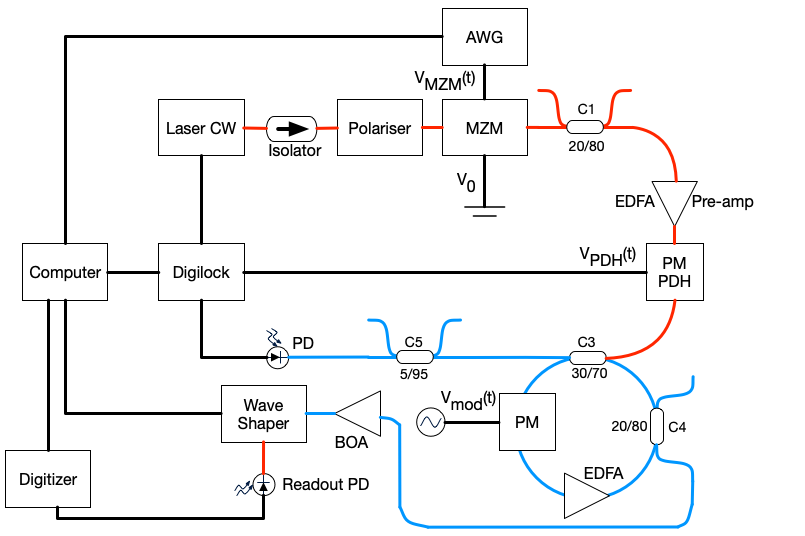
\includegraphics[width=\textwidth]{exp-setup}
	\caption{Schematic representation of the experimental setup for the \gls{wdm} reservoir computer experiment}
	\label{exp-setup}
\end{figure}

Let us start the presentation of the experiment by a general remark. On figure \ref{exp-setup}, the black lines represent electrical wires and the red lines optical fibres. The optical fibres used in the setup are polarisation maintaining single mode fibres.

% Mention only one PD

%%%%%%%%%% CHARACTERISATION OF THE RESERVOIR %%%%%%%%%%

\section{Characterisation of the reservoir}

%%% INTRODUCTION %%%

\subsection{Introduction}

%%% TRANSFER FUNCTION OF THE CAVITY %%%

\subsection{Transfer function of the cavity}

% MATHEMATICAL MODEL %

\subsubsection{Mathematical model}

% SIMULATIONS %

\subsubsection{Simulations}

% EXPERIMENTAL RESULTS %

\subsubsection{Experimental results}

%%% EFECTIVE LOSSES %%%

\subsection{Effective losses}

%%% MODULATION DEPTH %%%

\subsection{Modulation depth}

%%%%%%%%%% PDH STABILISATION TECHNIQUE %%%%%%%%%%

\section{Pound-Drever-Hall stabilisation technique}

%%% INTRODUCTION %%%

\subsection{Introduction}

%%% ERROR FUNCTION %%%

\subsection{Error function}

% MATHEMATICAL MODEL %

\subsubsection{Mathematical model}

% SIMULATION %

\subsubsection{Simulation}

% EXPERIMENTAL RESULTS %

\subsubsection{Experimental results}

%%%%%%%%%% CHARACTERISATION OF THE STABILISATION PERFORMANCE FOR DIFFERENT REGIMES %%%%%%%%%%

\section{Characterisation of the stabilisation performance for different regimes}

%%% INTRODUCTION %%%

\subsection{Introduction}

%%% APPROACH %%%

\subsection{Approach}

%%% RESULTS %%%

\subsection{Results}